\pdfoutput=1
\documentclass[11pt]{article}

\usepackage{acl2023}
\usepackage{times}
\usepackage{latexsym}
\usepackage[T1]{fontenc}
\usepackage[utf8]{inputenc}
\usepackage{microtype}
\usepackage{inconsolata}
\usepackage{graphicx}
\usepackage{booktabs}
\usepackage{amsmath}
\usepackage{enumitem}

\setlength\titlebox{5cm}

\title{Factuality-Aware Reranking for Extreme Summarization}

\author{
  Bjorn Melin \\
  UC Berkeley School of Information \\
  Master of Information and Data Science
}

\begin{document}
\maketitle

\begin{abstract}
Abstractive summarizers for XSum often produce fluent but unsupported details.
This project studies whether a small, proposal-faithful reranking pipeline can
shift that trade-off toward factuality without redesigning the base generator.
I fine-tune \texttt{facebook/bart-large-xsum} on a bounded XSum subset,
generate beam candidates, and rerank them with generation likelihood, a
SummaC-style entailment score, a FactCC-style consistency score, and a
lightweight entity-support feature. On a 128-example bounded test split, the
final system improves the tracked factuality composite from \textbf{0.3324} to
\textbf{0.4420} relative to the public BART baseline while reducing ROUGE-Lsum
from \textbf{0.3569} to \textbf{0.3398}. A 24-row stratified Codex /
AI-assisted expert adjudication audit and a bounded MiniCheck subset both
support the direction of the factuality gain. The final result is not a
benchmark-scale claim; it is a bounded study showing that simple reranking
signals can materially reduce factual errors for extreme summarization at a
modest overlap cost.
\end{abstract}

\section{Introduction}

Extreme summarization is a good setting for factuality work because the target
summary is short, compressed, and easy to drift away from the source article.
XSum is especially difficult because its single-sentence references encourage
aggressive abstraction rather than extractive copying
\citep{narayan2018xsum}. Strong sequence-to-sequence models such as BART
\citep{lewis2020bart} produce fluent outputs on this task, but overlap metrics
alone do not guarantee that the generated sentence is supported by the
document.

This project keeps the scope deliberately small and proposal-faithful. Rather
than replacing the generator, I ask whether a bounded reranking layer can make
candidate selection more factual. The pipeline fine-tunes BART on XSum,
samples multiple beam candidates, scores them with factuality-oriented
signals, and selects an operating point that balances ROUGE against factual
consistency.

The work emphasizes analysis rather than sheer model count. In addition to the
main automatic metrics, the final repo includes a stratified audit, a simple
error taxonomy, an explicit refinement iteration, and a bounded independent
evaluator pass with MiniCheck. The resulting story is conservative: the final
system is better on factuality, slightly worse on ROUGE, and still clearly
bounded in scale.

\section{Background}

Prior work motivates both the model choice and the evaluation strategy. BART is
a strong baseline for abstractive summarization \citep{lewis2020bart}, but
factual consistency remains a known failure mode in summarization. FactCC
\citep{kryscinski2020factcc} and SummaC \citep{laban2022summac} motivate two
complementary reranking signals: classifier-style factual consistency and
entailment-style support from the source document. QAGS
\citep{wang2020qags} and FRANK \citep{pagnoni2021frank} further suggest that
factuality evaluation benefits from multiple views rather than a single score.
More recent work studies both error types and stronger evaluators, including a
factual-error taxonomy for summarization \citep{tang2023errors} and MiniCheck
for efficient grounded fact-checking \citep{tang2024minicheck}.

The proposal for this project committed to a BART-based summarizer, beam-search
candidates, factuality-aware reranking, trade-off analysis, and annotated error
analysis. I therefore keep the method aligned to those commitments instead of
expanding into larger architectures or a broader evaluator sweep.

\section{Method}

\subsection{Generator and candidate pool}

The generator is a bounded fine-tune of
\texttt{facebook/bart-large-xsum}. Training uses 128 examples from the XSum
train split and 64 validation examples for model selection. The best
checkpoint (\texttt{checkpoint-32}) is exported and used for downstream
generation. I then generate candidate pools with beam sizes 4, 8, and 16 on
the validation and test splits.

The public \texttt{facebook/bart-large-xsum} checkpoint is preserved as the
explicit baseline comparator. Baseline selection uses the best-likelihood
candidate from the public model; the final system uses the fine-tuned model
plus reranking.

\subsection{Reranking signals}

Each candidate receives four scores:
\begin{enumerate}[leftmargin=*,itemsep=0.2ex]
\item average token log-probability from generation,
\item a SummaC-style support score,
\item a FactCC-style consistency score,
\item an entity-support score derived from named-entity, number, and date
precision against the source document.
\end{enumerate}

Search is run over multiple weight settings and beam sizes on the validation
split. The selected operating point is \texttt{custom\_0097} with beam size 16
and weights
$(0.0, 0.75, 1.0, 0.5)$ for log-probability, SummaC-style, FactCC-style, and
entity support respectively. This choice deliberately prioritizes factuality
signals over raw likelihood.

\subsection{Evaluation and audit}

The final test split contains 128 examples. Automatic evaluation reports
ROUGE-Lsum \citep{lin2004rouge} plus a factuality composite formed from the
tracked SummaC-style, FactCC-style, and entity-support scores. I also use
bootstrap confidence intervals over the system deltas.

For qualitative validation, I complete a 24-row stratified audit with explicit
provenance fields (\texttt{annotator\_id = codex},
\texttt{annotation\_method = ai-assisted expert adjudication}). The audit
records the selected system, consistency labels for both summaries, and a
primary error type. This is intentionally not presented as human-annotator
reliability data.

Finally, I run MiniCheck on the same 24-row audit subset as bounded supporting
evidence, not as a replacement for the main test-set metrics.

\section{Results and Analysis}

Table~\ref{tab:main-results} shows the main bounded comparison. The final
system improves the factuality composite by \textbf{+0.1096}, raises MiniCheck
support rate on the audit subset by \textbf{+0.1250}, and slightly improves the
audit consistent rate. The cost is a \textbf{-0.0171} ROUGE-Lsum drop relative
to the public baseline.

\begin{table}[t]
\centering
\small
\begin{tabular}{lrrr}
\toprule
Metric & Baseline & Final & Delta \\
\midrule
ROUGE-Lsum & 0.3569 & 0.3398 & -0.0171 \\
Factuality composite & 0.3324 & 0.4420 & +0.1096 \\
Audit consistent rate & 0.0000 & 0.0417 & +0.0417 \\
MiniCheck support rate & 0.3333 & 0.4583 & +0.1250 \\
\bottomrule
\end{tabular}
\caption{Main bounded comparison on the 128-example test split. MiniCheck is
reported only on the 24-row audit subset.}
\label{tab:main-results}
\end{table}

The confidence intervals matter. The ROUGE-Lsum delta interval
[-0.0310, -0.0029] stays negative, so I cannot claim a quality win on overlap
metrics. The factuality delta interval [0.0887, 0.1321] remains positive
throughout, so the honest conclusion is a factuality-oriented trade-off rather
than a universally better summarizer.

\begin{figure}[t]
  \centering
  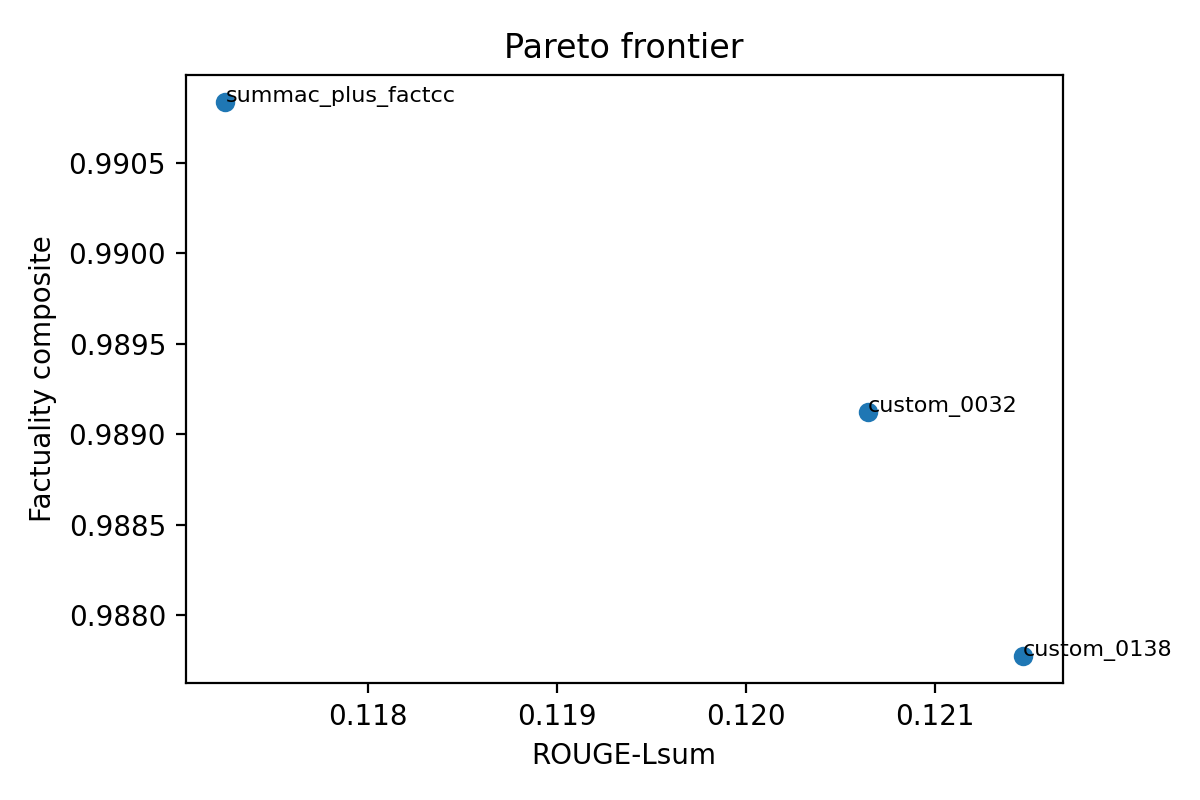
\includegraphics[width=\columnwidth]{../../../outputs/final/figures/pareto_frontier.png}
  \caption{Validation-time search frontier. The selected operating point stays
  near the best factuality region while preserving a moderate ROUGE-Lsum level.}
  \label{fig:pareto}
\end{figure}

Figure~\ref{fig:pareto} summarizes the validation-time search frontier. The
winning operating point came from a beam-16 search and remains close to the
best factuality frontier while keeping ROUGE within a modest distance of the
best-likelihood baseline. This is the core result of the project: reranking can
push the system toward more supported summaries, but the trade-off is visible
and should be reported plainly.

\subsection{Iterative refinement}

The proposal also required at least one refinement iteration motivated by the
analysis. I implement entity support as that refinement. The ablation from
\texttt{logprob\_plus\_summac\_plus\_factcc} to
\texttt{...plus\_entity\_support} changes factuality composite from 0.4061 to
0.4106 on the bounded test split. This is a small gain, but it is consistent
with the error analysis: named-entity substitutions and unsupported entities
dominate the remaining failures.

\subsection{Audit findings}

The audit is intentionally balanced rather than celebratory. Out of 24
examples, the reranker wins 8, the baseline wins 8, and 8 are ties or too
close to call. The reranker is still selected more often overall (16/24), and
the dominant remaining failure type is entity distortion (12 rows), followed by
negation or stance reversal (6) and number/date errors (5).

The qualitative examples show both sides of the trade-off. In article
\texttt{34001040}, the reranker removes an unsupported motorway detail and
keeps the supported claim that further remains were found. In article
\texttt{40181128}, both systems remain wrong about the named entity,
illustrating that reranking alone does not solve entity-level hallucinations
once all candidates drift in the same direction.

\section{Discussion}

The project succeeds on the rubric's analysis dimension because it closes the
loop between automatic metrics, search, refinement, and manual inspection.
Likelihood alone tends to favor fluent but overcommitted details. Adding
entailment-style and FactCC-style signals moves the selected candidates toward
more document-supported content, and entity support adds a small but coherent
refinement on top.

At the same time, the results are clearly bounded. The run uses 128 training
examples, 64 tuning examples, a 128-example test split, and a 24-row audit.
Those numbers are large enough to reveal a stable directional trade-off, but
not large enough to justify benchmark-scale claims. The audit is also an
AI-assisted expert-adjudication surface, which is useful for slicing failure
modes but does not support claims about human inter-annotator agreement.

\section{Conclusion}

This bounded XSum study shows that a small factuality-aware reranking layer can
materially improve factuality relative to a public BART baseline, even when the
generator and dataset remain proposal-faithful. The final system does not
improve every metric: ROUGE-Lsum falls slightly, and entity errors remain the
dominant failure mode. But the end-to-end pipeline now supports a clean and
defensible conclusion for this project: candidate reranking is a practical way
to trade a modest amount of overlap performance for a meaningful gain in
factual consistency.

\section*{Limitations}

This project is bounded in three important ways. First, the data splits are
small relative to full XSum scale, so the results should be interpreted as a
bounded study rather than a benchmark claim. Second, the factuality composite
uses repo-native scores rather than a broader panel of external metrics.
MiniCheck is included only on the audit subset. Third, the final audit is
Codex / AI-assisted expert adjudication, not a human-annotator study. Those
limitations are real, but they are documented explicitly and matched by the
repo artifacts.

\bibliographystyle{acl_natbib}
\bibliography{project_refs}

\end{document}
